\documentclass{article}
\usepackage[T1]{fontenc}
\usepackage{lmodern}
\usepackage{graphicx}
\usepackage{amsmath,amssymb}
\usepackage[a4paper,margin=2cm]{geometry}
\usepackage[absolute,overlay]{textpos}
\setlength{\TPHorizModule}{1mm}
\setlength{\TPVertModule}{1mm}
\usepackage[indonesian]{babel}
\usepackage{hyperref}
\setlength{\emergencystretch}{2em}
% unit: Halaman 29

\begin{document}

% === Halaman 29 (llm) ===

\begin{itemize}
    \item Contoh lain: Kurva eliptik $y^2 \equiv x^3 + x + 1 \pmod{23}$ memiliki titik-titik di dalam himpunan $\{(0, 1), (0, 22), (1, 7), (1, 16), (3, 10), (3, 13), (5, 4), (5, 19), (6, 4), (6, 19), (7, 11), (7, 12), (9, 7), (9, 16), (11, 3), (11, 20), (12, 4), (12, 19), (13, 7), (13, 16), (17, 3), (17, 20), (18, 3), (18, 20), (19, 5), (19, 18)\}$.
\end{itemize}

\vspace{10mm}

% deskripsi: Grafik scatter plot yang menunjukkan titik-titik solusi dari persamaan kurva eliptik $y^2 \equiv x^3 + x + 1 \pmod{23}$ pada bidang koordinat x dan y.
% bbox normalisasi: [0.2040, 0.3210, 0.7680, 0.8560]
\begin{textblock*}{118.44mm}(42.84mm,95.34mm)
\noindent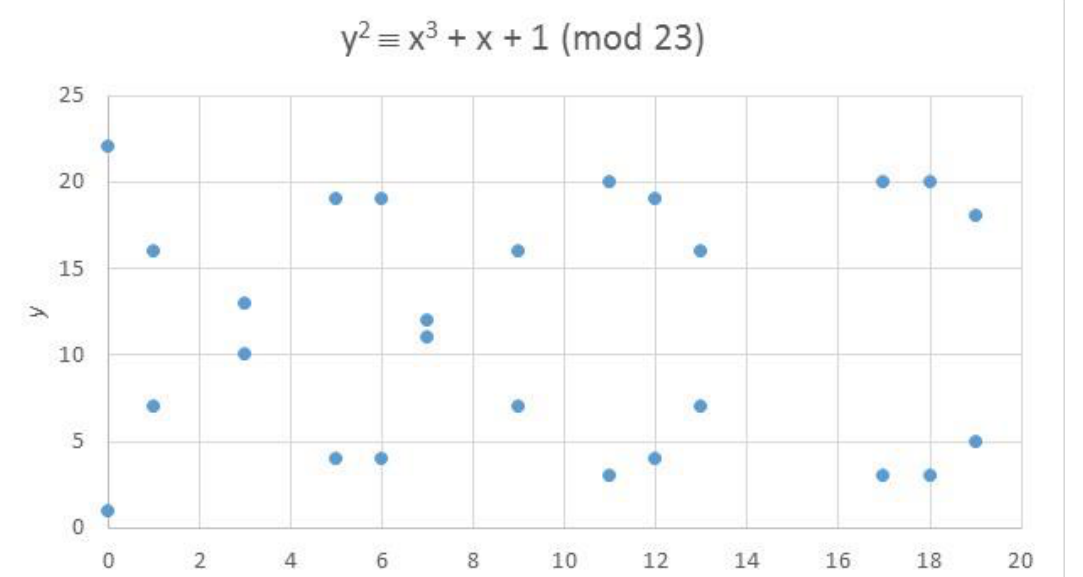
\includegraphics[width=118.44mm,height=158.89mm]{../../images/llm/page_029_img_01.png}%
\end{textblock*}

\end{document}
